\documentclass[11pt,a4paper]{article}
\usepackage{amsmath}
\usepackage{amsfonts}
\usepackage{amssymb}
\usepackage{fancyhdr}
\usepackage{lastpage}
\usepackage{graphicx}
\usepackage{ucs}
\usepackage[utf8x]{inputenc}
\usepackage[italian]{babel}
\usepackage[colorlinks=true,linkcolor=black]{hyperref}

\renewcommand{\headrulewidth}{0.6pt}
\renewcommand{\footrulewidth}{0.6pt}
% impostazione dello stile per le pagine interne del documento
\lhead{\leftmark}
\chead{}
\rhead{
\includegraphics[scale=0.15]{logo.png} }
\lfoot{Manuale Utente - Docente v0.4.0}
\cfoot{}
\rfoot{\thepage \ di \pageref{LastPage}}
% ridefinizione dello stile plain per il frontespizio
\fancypagestyle{plain}{
\fancyhf
}
% impostazione dello stile per l'indice
\fancypagestyle{indice}{
\lhead{\leftmark}
\chead{}
\rhead{
\includegraphics[scale=0.15]{logo.png}}
\lfoot{Manuale Utente v0.4.0}
\cfoot{}
\rfoot{}
}
\headheight = 46pt
%definizione del comando "\modfiche" per la creazione del diario delle modifiche
\newcommand{\modifiche} 
{
\newpage
\begin{center}
\textbf{Diario delle modifiche} \\
\bigskip
\begin{tabular}{|c|c|p{0.62\textwidth}|}
\hline
\textsc{Data} & \textsc{Versione} & \textsc{Modifica} \\
\hline
\hline
\textit{05-03-2009} & 0.4.0 & Inserito il Glossario\\
\hline
\textit{03-03-2009} & 0.3.0 & Completata la Descrizione funzionale e le Azioni richieste-permesse\\
\hline
\textit{26-02-2009} & 0.2.0 & Inserite la premessa e le sezioni Introduzione e Descrizione Generale\\
\hline
\textit{24-02-2009} & 0.1.0 & Stesura indice\\
\hline
\end{tabular}
\end{center}
}
%definizione del comando "\info" per la creazione delle informazioni del documento
\newcommand{\info} {
\bigskip
\begin{tabbing}
	\hspace*{0.3\textwidth} \= \hspace*{0.5\textwidth} \kill
	\parbox{0.3\textwidth}{\textbf{Verifica: }} \> \parbox{0.5\textwidth}{} \\
	\parbox{0.3\textwidth}{\textbf{Approvazione: }} \> \parbox{0.5\textwidth}{} \\
	\parbox{0.3\textwidth}{\textbf{Stato: }} \> \parbox{0.5\textwidth}{Formale} \\
	\parbox{0.3\textwidth}{\textbf{Uso: }} \> \parbox{0.5\textwidth}{Esterno} \\
	\parbox{0.3\textwidth}{\textbf{Distribuzione: }} \> \parbox{0.5\textwidth}{QuiXoft} \\
							\> \parbox{0.5\textwidth}{Rossi Francesca} \\
							\> \parbox{0.5\textwidth}{Vardanega Tullio} \\
							\> \parbox{0.5\textwidth}{Conte Renato} \\
\end{tabbing}
}
%definizione del comando "\frontespizio" per la creazione del frontespizio
\newcommand{\frontespizio} {
\thispagestyle{plain}
\title{\begin{Huge}\textsc{Progetto SIGEOL}\end{Huge} \\ \textit{Manuale Utente - Docente\\ v0.4.0}}
\author{Redazione: Scortegagna Carlo}
\maketitle
\medskip
\begin{center}

\includegraphics[scale=0.5]{logo.png} \\
\textit{quixoft.sol@gmail.com} \\
\end{center}
\medskip
\info
\begin{center}
\textbf{Sommario} \\
Manuale utente per l'utilizzo del progetto \textit{SIGEOL} da parte dei docenti, contenente la spiegazione di tutte le funzionalità disponibili, dei possibili problemi e delle relative soluzioni.
\end{center}
\newpage
}
%definizione del comando "\indice" per la creazione dell'indice
\newcommand{\indice} {
\thispagestyle{indice}
\tableofcontents
\newpage
}
\pagestyle{fancy}
\begin{document}
\frontespizio
\indice
\setcounter{page}{1}
\section{Premessa}
L'utilizzo del progetto software SIGEOL è previsto da 3 differenti tipologie d'utenti:
\begin{enumerate}
 \item Utenti che non abbiano effettuato il \underline{login} (in seguito riferiti come visitatori) che accedono al sistema solo per consultare informazioni
 \item Docenti che abbiano accreditato la propria identità tramite login
 \item Segreteria Didattica che accede al sistema tramite login
\end{enumerate}
\bigskip
Le funzionalità offerte ai visitatori sono solamente di consultazione di informazioni: possono consultare lo schema d'orario dei diversi corsi di laurea, possono accedere alle informazioni relative ai docenti, alle aule, agli edifici, agli insegnamenti, ecc...

Tali funzioni sono state ritenute talmente di immediato utilizzo ed esenti da possibili problematiche che il team QuiXoft ha ritenuto superflua la redazione di un manuale utente dedicato ai visitatori.
E' stata presa questa decisione anche meditando sul largo numero di utenti visitatori che accederanno al progetto SIGEOL: una cosi grande diffusione di un eventuale manuale utente dedicato a loro sarebbe stata infattibile.

Le operazioni dedicate solamente ai visitatori saranno invece ampiamente commentate e descritte proprio all'interno dell'interfaccia grafica, per facilitare la consultazione delle varie informazioni ai visitatori senza che questi debbano leggere un eventuale manuale utente.

\bigskip \bigskip
Data la gran diversità delle operazioni accessibili dalle due rimanenti tipologie d'utenza, saranno redatti due distinti manuali utente: i docenti dovranno consultare il documento \textsc{Manuale Utente Docente}, la segreteria didattica invece dovrà consultare il \textsc{Manuale Utente Segreteria Didattica}.

Caso particolare a quanto appena affermato è il Presidente del CCS: avendo a disposizione sia le funzioni dedicate ai docenti sia quelle dedicate alla segreteria didattica, per questo utente del sistema SIGEOL è consigliata la consultazione di entrambi i manuali.
\newpage
\section{Introduzione}
\subsection{Definizione dell'utente del prodotto}
Il presente manuale utente è rivolto alla spiegazione delle diverse funzionalità del sistema SIGEOL dedicate ai docenti.
L'accesso alle operazioni descritte in seguito è possibile solamente dopo aver effettuato con successo il login al sistema, confermando di avere i privilegi assegnati ai docenti.

Sia prima sia dopo aver effettuato il login, sono sempre disponibili anche le funzioni di consultazione informazioni dedicate agli utenti visitatori, ampiamente descritte all'interno dell'interfaccia grafica, e quindi non illustrate nel presente documento.
\subsection{Come leggere il manuale}
Il presente manuale descrive brevemente le parti pubbliche del progetto (vedi sezione `Descrizione Generale`) e si focalizza in seguito sulle funzionalità private dedicate ai docenti (sezione `Azioni Richieste - Permesse`).

Saranno illustrate e descritte tutte le possibili operazioni effettuabili, con l'aiuto di \underline{screenshot} qualora ve ne fosse la necessità.
Per non appesantire troppo la lettura e la consultazione del presente manuale utente, alcune funzionalità che il team QuiXoft ha ritenuto di facile comprensione non sono accompagnate da screenshot.

Proseguendo con la lettura, saranno elencati i vari errori a cui si potrà andare incontro utilizzando il progetto SIGEOL, e le eventuali soluzioni per porvi rimedio.

Il manuale termina con un Glossario, contenente la spiegazione di alcuni termini usati nel corso di questo documento.
I termini che possiedono una descrizione all'interno del Glossario saranno riconoscibili perchè presentano una \underline{sottolineatura}.

\subsection{Come riportare problemi e malfunzionamenti}
La segnalazione di problemi o manfulzionamenti del sistema SIGEOL andrà fatta inviando un email all'indirizzo \textit{quixoft.sol@gmail.com}.
Quest'ultima dovrà contenere le seguenti informazioni:
\begin{itemize}
 \item Nome e cognome del mittente
 \item Data e ora in cui il problema si è manifestato
 \item Tipo d'utenza
 \item Informazioni sull'ambiente in cui è stato rilevato l'errore (sistema operativo, \underline{browser}, ecc...) o qualsiasi altra informazione d'utilità ritenuta importante dal mittente (configurazione hardware, risoluzione dello schermo, ecc...)
 \item Descrizione del malfunzionamento riscontrato, dei messaggi d'errore visualizzati, delle eventuali operazioni svolte prima del manifestarsi del problema.
\end{itemize}
Le segnalazioni saranno prese in considerazione il prima possibile e i problemi riscontrati saranno risolti al più presto dai membri del team QuiXoft.
\section{Descrizione generale}
Il progetto SIGEOL si presenta all'utente come un semplice sito internet, la cui consultazione è similare e non presenta difficoltà rispetto ai canoni classici delle pagine che compongono il \underline{World Wide Web}.

Tale sito è raggiungibile utilizzando un qualsiasi elaboratore connesso ad internet: l'unico software necessario per la sua consultazione è un semplice browser (come, ad esempio, Firefox, Internet Explorer, Chrome, Safari, Opera, ecc...).

L'effettivo indirizzo internet a cui raggiungere il sito del progetto SIGEOL non è al momento noto con certezza e non verrà di conseguenza menzionato nel presente documento: sarà compito del Committente scegliere e predisporre tale indirizzo.

Una volta digitato l'indirizzo internet corretto nel browser sarà visualizzata la pagina principale del progetto, contenente le prime informazioni e i \underline{link} alle altre pagine disponibili.

Prima di effettuare il login saranno disponibili e visualizzate solamente le pagine pubbliche, che consentono di consultare:
\begin{itemize}
 \item orari di lezione per i vari corsi di laurea presenti
 \item informazioni riguardanti i suddetti corsi di laurea e gli insegnamenti
 \item informazioni personali e contatti dei docenti assegnati ai vari insegnamenti
 \item informazioni sugli edifici e sulle aule presenti
\end{itemize}
Sarà inoltre possibile generare un file in formato \underline{Pdf} con l'orario richiesto, per poterlo facilmente stampare o salvare localmente.

Come detto in precedenza, le funzioni appena elencate sono di immediato utilizzo e non verrano quindi spiegate esaustivamente nel presente documento.
Una semplice spiegazione del loro funzionamento sarà presente direttamente all'interno delle relative pagine del sito web del progetto.

\bigskip
Una volta effettuato il login con l'indirizzo email e la password scelta in fase di registrazione, saranno disponibili anche tutte le funzioni private del sito riservate ai docenti:
\begin{itemize}
 \item modifica dei dati personali inseriti in fase di registrazione
 \item inserimento vincoli e preferenze
 \item cambio password
\end{itemize}
Le funzioni appena elencate saranno accuratamente illustrate nel proseguire del presente documento.
\subsection{Interfaccia grafica}
Allo stato attuale, il progetto è funzionante e testato in ogni sua parte.
Nonostante ciò, il layout grafico che andrà utilizzato nella versione finale del prodotto non è ancora stata sviluppato: è presente solamente un interfaccia grafica di prova, per testare e valutare le varie funzionalità del progetto.

L'aspetto grafico che il sito internet assumerà al momento del suo rilascio verrà deciso in collaborazione con il Committente, per adeguarsi allo stile delle pagine internet già in suo possesso o per adattarsi ai suoi gusti.

Il \underline{template} attuale è da ritenersi quindi esclusivamente temporaneo e, di conseguenza, le immagini consultabili all'interno del presente documento non hanno velleità di essere definitive, ma andranno aggiornate al momento della scelta dell'aspetto grafico definitivo del sito internet.
\section{Istruzioni per l'uso}
\subsection{Descrizione funzionale}
\subsubsection{Pagina Principale}
La pagina principale del prodotto SIGEOL presenta la possibilità di consultare tutte le informazioni pubbliche. Il numero e il raggruppamento dei link a tali pagine verrà deciso al momento della scelta dell'aspetto grafico definitivo del sito internet.

Sarà inoltre presente un link che porta alla pagina di login, in cui si potranno inserire il proprio indirizzo email e la propria password per accedere alle aree e alle funzioni private riservate ai docenti.
\subsubsection{Pagina di Login}

\begin{center}
	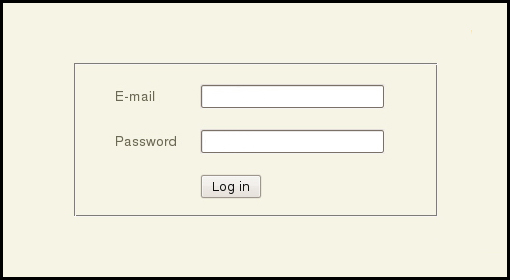
\includegraphics[scale=0.5]{images/login.jpg}\\
	\textbf{fig. 4.1.2.1} Form di login\\
\end{center}

La pagina di login, come si vede in figura 4.1.2.1, offre la possibiltà agli utenti come la segreteria didattica o i docenti di inserire il proprio username (corrispondente all'indirizzo email) e la relativa password per poter accedere alle funzioni private messe a loro disposizione.

In caso di login corretto verrà visualizzata nuovamente la pagina principale del prodotto SIGEOL, con in più i link a tutte le funzioni private accessibili.
In caso di errore nell'inserimento dell'indirizzo email o della password verrà visualizzato un messaggio di notifica di tale errore, come in figura 4.1.2.2.
Sarà immediatamente possibile reinserire i dati corretti e ritentare il login.

\begin{center}
	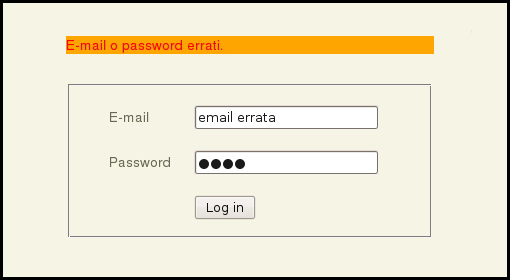
\includegraphics[scale=0.5]{images/login_errato.jpg}\\
	\textbf{fig. 4.1.2.2} Form dopo un login errato\\
\end{center}

Le funzioni accessibili alle due tipologie di utenti appena citate sono diametralmente opposte: nei successivi capitoli del presente documento verranno quindi solamente illustrate le funzioni dedicate ai docenti.
\subsection{Azioni richieste/permesse}
Ogni capitolo di questa sezione si riferisce ad una particolare funzione che il sistema SIGEOL mette a disposizione dei docenti.
\subsubsection{Registazione docente}
Prima di poter effettuare il login e accedere alle funzionalità riservate, è necessario che ogni docente si registri al sistema SIGEOL.

Non è possibile registrarsi al sistema senza essere stati preventivamente invitati dalla segreteria didattica, ne è presente all'interno del sito del progetto SIGEOL un link alla funzione di iscrizione.

\begin{center}
	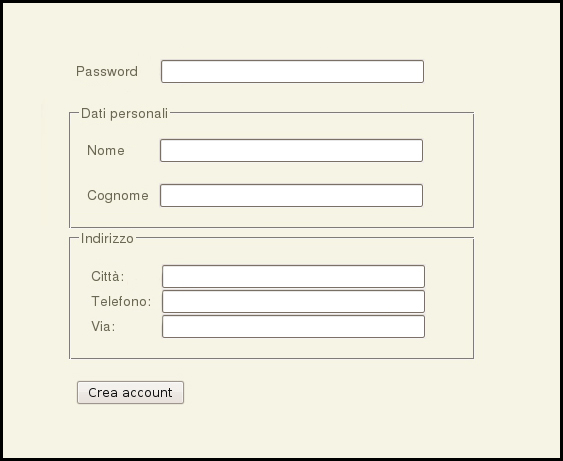
\includegraphics[scale=0.5]{images/registrazione_docente.jpg}\\ 
	\textbf{fig. 4.2.1.1} Form di registrazione docenti\\
\end{center}

L'unica modalità per completare la registrazione è seguire il link che verrà spedito alla casella di posta elettronica di ogni docente invitato dalla segreteria didattica. Questo link porta alla form illustrata in figura 4.2.1.1, in cui si dovranno inserire i seguenti dati:
\begin{itemize}
 \item password: non deve essere vuota e deve contenere come minimo 6 numeri o caratteri, sia maiuscoli sia miniscoli. Da notare che uno stesso carattere maiuscolo e minuscolo è considerato differente dal sistema: si prega quindi di prestare attenzione al momento della scelta della password.
 \item nome: deve semplicemente essere composto da caratteri.
 \item cognome: segue le stesse regole relative al nome.
 \item città: il nome della città deve essere composto solamente da caratteri o spazi. La lunghezza massima è fissata in 30 caratteri.
 \item numero di telefono: deve essere inserito nel formato `prefisso-numero`. Il prefisso può essere composto solamente da numeri e la sua lunghezza può variare da 2 a 4. Anche il numero segue le stesse regole, ma la lunghezza dev'essere compresa tra 6 e 8 cifre.
 \item via: si accettano caratteri, numeri e spazi. In questo caso la lunghezza massima è fissata in 50 caratteri, compresi gli spazi.
\end{itemize}
Una volta inseriti correttamente tutti i dati richiesti, è sufficiente premere il pulsante `Crea Account` per completare la registrazione.

D'ora in poi sarà possibile accedere al sistema SIGEOL completando il login con il proprio indirizzo e-mail e la password appena scelta.
\subsubsection{Modifica dei dati personali}
I dati personali inseriti in fase di registrazione possono essere cambiati in ogni momento seguendo il link `Modifica dati personali`, visibile e accessibile solamente dopo aver effettuato con successo il login.

I dati che è possibile aggiornare sono gli stessi inseriti in fase di registrazione, eccezion fatta per la password, che ha a disposizione una funzione di aggiornamento dedicata. Le regole da seguire per il completamento dei campi sono le stesse sopra illustrate per la funzionalità di registrazione.
\subsubsection{Cambio Password}
La pagina di cambio password permette semplicemente di modificare la password del proprio \underline{account}.

La procedura è particolarmente semplice: è sufficiente inserire la nuova password e premere il pulsante `Cambio Password`, come illustrato in figura 4.2.3.1.

\begin{center}
	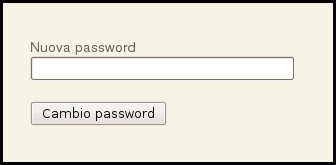
\includegraphics[scale=0.5]{images/cambio_password.jpg}\\
	\textbf{fig. 4.2.3.1} Form di cambio password\\
\end{center}

\subsubsection{Inserimento vincoli e preferenze}
La pagina di inserimento vincoli e preferenze permette di inserire degli intervalli temporali in cui il docente non può tenere una lezione oppure preferisce non tenere una lezione. La differenza tra i due casi viene dettagliatamente spiegata nelle sezioni a seguire.

Tale pagina contiene una lista dei vincoli e delle preferenze inseriti precedentemente dal docente, che potranno essere modificati o cancellati selezionando rispettivamente i link `Modifica` o `Elimina` presenti a fianco di ogni vincolo e di ogni preferenza.

Oltre alla sopracitata lista, nella pagina è notificata anche una data entro la qualche è obbligatorio aver inserito tutti i propri vincoli e preferenze: scaduta questa data, opportunamente fissata dalla segreteria didattica prima dell'inizio di un nuovo periodo di lezione, non sarà più possibile inserire nuovi vincoli.

Tale data verrà aggiornata nel momento in cui la segreteria deciderà di riaprire la possibilità di inserimento di vincoli e preferenze per il periodo successivo.

Da notare che i vincoli e le preferenze inserite in un periodo precedente rimarranno memorizzati anche per il periodo successivo: se non fossero più validi o non fossero più necessari, è sufficiente eliminarli o modificarli.

Sono messe anche a disposizione le due funzionalità `Nuovo Vincolo` e `Nuova Preferenza`, illustrate qui di seguito.
\newline \newline \newline
\begin{large}\textbf{Inserimento nuovo vincolo:}\end{large}
\newline \newline
Un docente è tenuto ad inserire un vincolo di indisponibilità qualcora, per validi motivi, in qualche determinato giorno o in qualche determinata ora non potesse assolutamente tenere delle lezioni per gli insegnamenti a lui assegnati.

I vincoli inseriti all'interno del sistema SIGEOL verranno automaticamente accettati e categoricamente rispettati nel calcolo dell'orario delle lezioni.
Nel caso il sistema non riesca a generare l'orario delle lezioni rispettando tutti i vincoli inseriti da tutti i docenti, sarà compito della segreteria didattica o del presidente del CCS rilassare uno o più vincoli, o chiedere ai rispettivi docenti di modificare o eliminare un determinato vincolo.

Al momento dell'inserimento, i vincoli devono essere dotati di un opportuna motivazione, che sarà consultabile dalla segreteria didattica e dal presidente del CCS per valutarne la validità.

I campi dato da completare nel momento dell'inserimento di un nuovo vincolo sono:
\begin{itemize}
 \item scelta del giorno della settimana, tramite menu a tendina.
 \item scelta dell'intervallo orario: se l'indisponibilità dura tutto la giornata si prega di selezionare l'opzione `Tutto il giorno`, altrimenti è necessario selezionare l'ora di inizio e l'ora di fine dell'indisponibilità.
 \item motivazione: è obbligatorio inserire una sintetica motivazione dell'indisponibilità. E' possibile usare indistintamente caratteri, simboli o numeri.
\end{itemize}
Al termine dell'inserimento di tutti i dati è sufficiente premere il pulsante `Salva` per memorizzare il vincolo all'interno del sitema SIGEOL: d'ora in poi tale vincolo verrà rispettato nel calcolo dell'orario delle lezioni.
\newline \newline \newline
\begin{large}\textbf{Inserimento nuova preferenza:}\end{large}
\newline \newline
Un docente è tenuto ad inserire una preferenza nel caso abbia dei giorni o degli orari in cui preferisce non tenere delle lezioni: la differenza rispetto ai vincoli è che questi ultimi vengono sicuramente rispettati nel calcolo dell'orario, mentre le preferenze vengono rispettate solamente nel caso non ci siano altri fattori con priorità maggiore ad intralciarle.

E' possibile inserire quante più preferenze si vogliono, senza la necessità di inserire una motivazione.

Si raccomanda all'utente di meditare bene se un proprio periodo di indisponibilità sia un vincolo o sia una preferenza, e di limitare al massimo l'utilizzo della sopra illustrata funzionalità di `Inserimento nuovo vincolo`, per non limitare troppo le disponibilità degli altri docenti e non rendere difficoltosa la generazione di un orario di lezione che soddisfi le esigenze di tutti.

I campi dato da completare nel momento dell'inserimento di una nuova preferenza sono:
\begin{itemize}
 \item scelta del giorno della settimana, tramite menu a tendina.
 \item scelta dell'intervallo orario: se l'indisponibilità dura tutto la giornata si prega di selezionare l'opzione `Tutto il giorno`, altrimenti è necessario selezionare l'ora di inizio e l'ora di fine dell'indisponibilità.
\end{itemize}
Al termine dell'inserimento di tutti i dati è sufficiente premere il pulsante `Salva` per memorizzare la preferenza all'interno del sitema SIGEOL.

\subsection{Errori probabili e cause possibili}
L'inserimento dei dati nelle varie form da parte della segreteria didattica è seguito passo passo dal sistema SIGEOL: ogni dato è controllato e validato prima di essere salvato in modo persistente.

E' pertanto difficile, se non impossibile, inserire dati errati senza che questo venga segnalato.
La segnalazione degli errori avverrà in seguito alla pressione del pulsante di invio dei dati: verrà quindi visualizzata nuovamente la form da cui si era partiti, con in più la segnalazione dell'errore. Sarà quindi sufficiente correggere il dato che ha generato l'errore e premere nuovamente il pulsante di invio dei dati (che potrà essere `Salva`, `Salva Modifiche` o altro, in base alla form su cui si sta lavorando).

Per non andare incontro a segnalazioni continue di errori è necessario seguire le linee guida indicate nella sezione `Azioni richieste - permesse` del presente documento, di volta in volta consultando la sottosezione relativa alla funzionalità che si sta usando.

Si è deciso di non elencare tutti i possibili messaggi d'errore, in quanto tali messaggi sono talmente chiari e autoesplicativi da non necessitare di ulteriori definizioni.
\newpage
\section{Appendice}
\subsection{Glossario}
\flushleft \Huge A \bigskip
\hrule
\smallskip
\normalsize
\begin{description}
	\item[Account:] insieme di funzionalità, strumenti e contenuti attribuiti ad un utente in determinati contesti operativi. In informatica, attraverso il meccanismo dell'account, il sistema mette a disposizione dell'utente un ambiente con contenuti e funzionalità personalizzabili, oltre ad un conveniente grado di isolamento dalle altre utenze parallele.
\end{description}
\bigskip
\Huge B \bigskip
\hrule
\smallskip
\normalsize
\begin{description}
	\item[Browser:] software che consente agli utenti di visualizzare e interagire con testi, immagini e altre informazioni, tipicamente contenute in una pagina web di un sito. Il browser è in grado di interpretare il codice HTML (e più recentemente XHTML) e visualizzarlo in forma di ipertesto. L'HTML è il codice col quale la maggioranza delle pagine web nel mondo sono composte: il web browser consente perciò la navigazione nel web.
\end{description}
\bigskip
\Huge L \bigskip
\hrule
\smallskip
\normalsize
\begin{description}
	\item[Link:] letteralmente indica un collegamento. In informatica è usato per indicare l'indirizzo web di una risorsa.
	\item[Login:] termine inglese per indicare la procedura di accesso ad un sistema o un'applicazione informatica.
	\item[Logout:] termine inglese per indicare la procedura di uscita da un sistema o un'applicazione informatica.
\end{description}
\bigskip
\Huge P \bigskip
\hrule
\smallskip
\normalsize
\begin{description}
	\item[Pdf:] il Portable Document Format, comunemente abbreviato Pdf, è un formato di file basato su un linguaggio di descrizione di pagina sviluppato da Adobe per rappresentare documenti in modo indipendente dall'hardware e dal software utilizzati per generarli o per visualizzarli. Ogni documento redatto dal team QuiXoft viene esportato in questo formato.
\end{description}
\bigskip
\Huge S \bigskip
\hrule
\smallskip
\normalsize
\begin{description}
	\item[Screenshot:] termine inglese (da screen, schermo, e shot, scatto fotografico) che indica l'istantanea di ciò che visualizzato in un determinato istante sullo schermo di un elaboratore.
\end{description}
\bigskip
\Huge T \bigskip
\hrule
\smallskip
\normalsize
\begin{description}
	\item[Template:] documento o programma dove, come in un foglio semicompilato cartaceo, su una struttura generica o standard esistono spazi temporaneamente "bianchi" da riempire successivamente.
\end{description}
\bigskip
\Huge W \bigskip
\hrule
\smallskip
\normalsize
\begin{description}
	\item[World Wide Web:] termine di origine inglese, in sigla WWW e spesso abbreviato in Web, è uno dei servizi di Internet, la più grande rete ad accesso pubblico di computer mai realizzata. In particolare il Web è, assieme alla posta elettronica, il servizio di Internet più utilizzato e conosciuto.
\end{description}
\modifiche
\end{document}
